\section{Creazione del training set}
Il dataset in input è stato prodotto a seguito delle operazioni di data integration su tre dataset originari. Durante queste operazioni, gli attributi privi di informazioi rilevanti ai fini dell'addestramento di un modello di Machine Learning sono stati rimossi, ottenendo un dataset già pronto all'uso. Per dividere il dataset in train set e test set, è stata definita una funzione ad hoc che permette di dividere il dataset in 10 parti, usandone poi 9 per il trainset e la restante per il testset. Questa funzione si è rivelata fondamentale per l'operazione di 10-fold cross validation, in cui il modello viene addestrato e testato su porzioni differenti del dataset.

\section{Analisi esplorativa del dataset}
\todo{Controllare eventiali affermazioni "forti" MM}
\todo{Posizionamneto figure MM}
Ai fini di evidenziare la distribuzione dei dati rispetto ai vari attributi del dataset, è stata condotta un'analisi esplorativa del dataset mediante funzioni statistiche del linguaggio R.\\
I dataset è formato da 312895 sample, 7 feature e una etichetta a 2 livelli.
Tramite la funzione \texttt{sapply(dataset, class)} è stata ottenuta la classe di ogni feature, che è stata poi sottoposta ad un'analisi più approfondita.\\
L'attributo Country è un attributo stringa fattorizzato, che presenta 21 livelli. Il valore più frequentemente riportato è "United States", seguito da "United Kindom" e "Canada".\\
L'attributo GDP per capita è un attributo numerico di valore intero continuo che rappresenta il guadagno annuo medio nello stato in cui il progetto è stato proposto. La distribuzione dei due attributi sopracitati è mostrata in Figura \ref{fig:countrygdp}. Notiamo che per entrambi i grafici è stata utilizzata la scala logaritmica, in quanto la frequenza associata ad alcuni valori è molto alta. In particolare abbiamo notato che la maggior parte dei progetti (oltre il 70\%) è stato creato negli Stati Uniti.

\begin{figure}%
	\centering
	\subfloat[Distribuzione dell'attributo Country. Si noti che l'asse y è riportato in scala logaritmica.]{{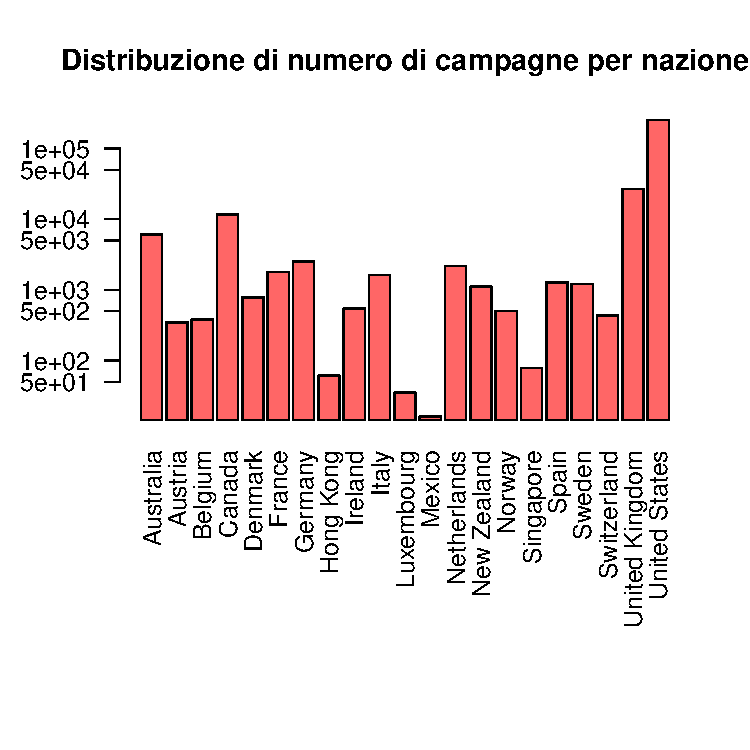
\includegraphics[width=0.45\linewidth]{../FinalResults/Images/Data_exploration_plots/barlpot_country} }}%
	\qquad
	\subfloat[Distribuzione dell'attributo rappresentante il GDP pro capite]{{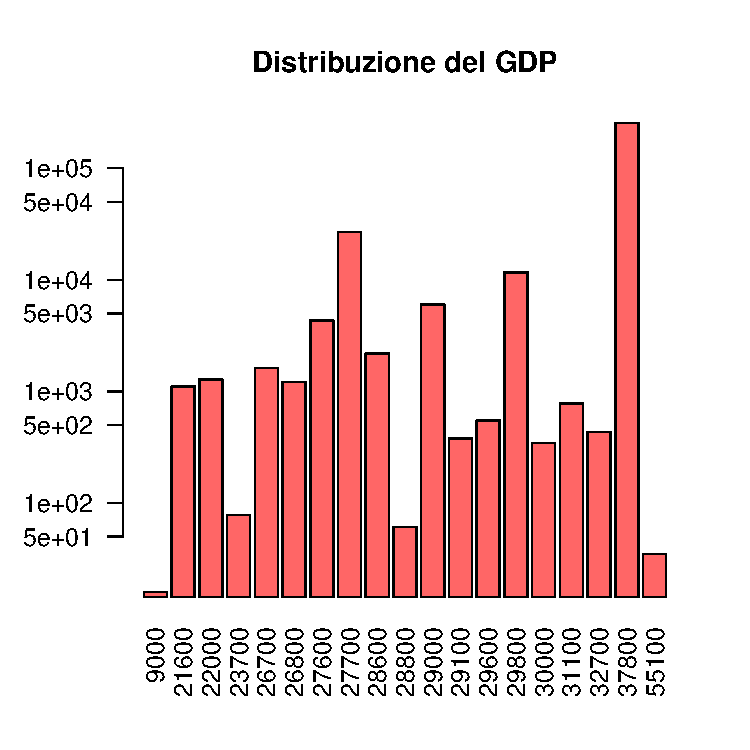
\includegraphics[width=0.45\linewidth]{../FinalResults/Images/Data_exploration_plots/barlpot_gdp}}}%
	\caption{}%
	\label{fig:countrygdp}%
\end{figure}

Sono poi stati analizzati gli attributi relativi alle categorie dei progetti proposti, quindi le feature main category e category. Entrambi i campi, costituiti da stringhe fattorizzate, si mostrano distribuite in modo sostanzialmente uguale tra i possibili valori, come mostrato nella Figura \ref{fig:piecategory}. 

\begin{figure}%
	\centering
	\subfloat[Distribuzione dell'attributo rappresentante la categoria specifica del progetto.]{{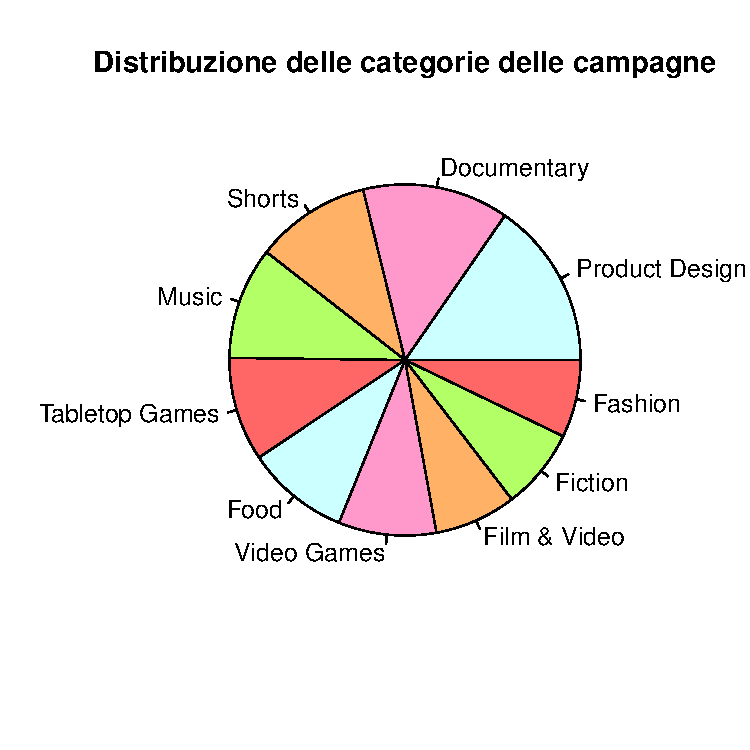
\includegraphics[width=0.45\linewidth]{../FinalResults/Images/Data_exploration_plots/pie_categories} }}%
	\qquad
	\subfloat[Distribuzione dell'attributo rappresentante la categoria generale del progetto.]{{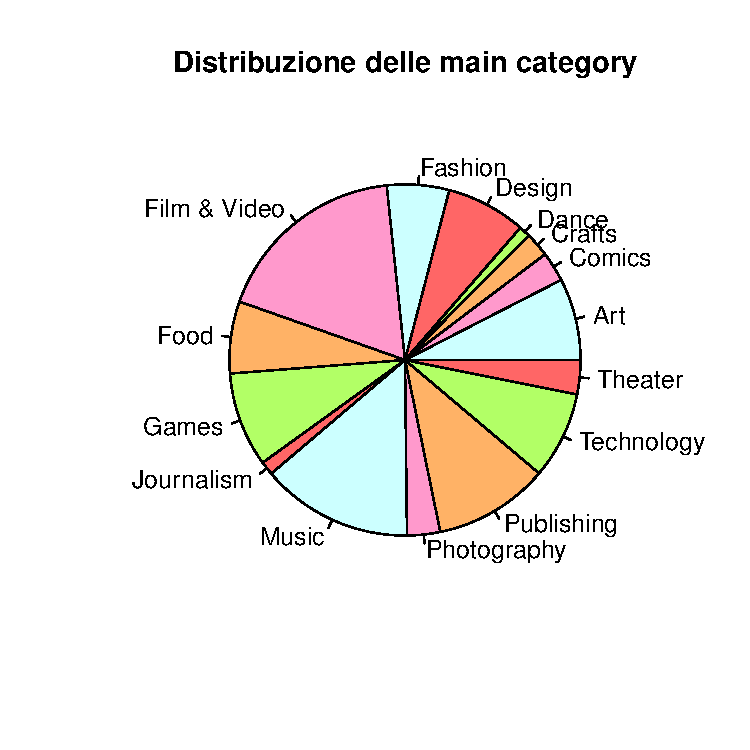
\includegraphics[width=0.45\linewidth]{../FinalResults/Images/Data_exploration_plots/pie_main_category}}}%
	\caption{}%
	\label{fig:piecategory}%
\end{figure}

La distribuzione del campo service ( sezione a della Figura \ref{fig:piestate}), rappresentante la percentuale di sviluppo dei settori terziari nel paese in cui è stato proposto il progetto, mostra come la maggior parte dei sample sia relativa a paesi con un settore terziario predominante sugli altri due.   


Le feature goal e backer sono due attributi interi e continui che rappresentano rispettivamente la richiesta minima di denaro al fine di considerare il progetto riuscito ed il numero di donatori. Per questi due campi sono stati analizzati il valore medio e la deviazione standard; i risultati ottenuti sono stati riportati nella Tabella \ref{tab:meansdgoalbackers}. Un valore così elevato di deviazione standard rispetto alla media, indica che i dati sono caratterizzata da una significativa varietà e distanza dal valore medio riportato.
\begin{table}
	\centering
	\label{tab:meansdgoalbackers}
	\caption{Media e deviazione standard degli attributi goal e backers}
	\begin{tabular}{|c|c|c|}
		\hline 
		\textbf{Feature} & \textbf{Valore medio} & \textbf{Deviazione standard} \\ 
		\hline 
		goal & 46672.68 & 1112774 \\ 
		\hline 
		backers & 102.98 & 946.76 \\ 
		\hline 
	\end{tabular} 
\end{table}


L'ultimo aspetto analizzato è stata la distribuzione dell'etichettatura dei progetti, per capire come fossero divise le tuple all'interno del nostro dataset. Come mostrato nella sezione b della Figura \ref{fig:piestate}, la maggioranza dei sample (63\%) in nostro possesso risultano essere relativi a progetti fallimentari. Il numero non risulta comunque tanto squilibrato da generare problemi nella fase di addestramento dei modelli di Machine Learning.

\begin{figure}%
	\centering
	\subfloat[Distribuzione dell'attributo service.]{{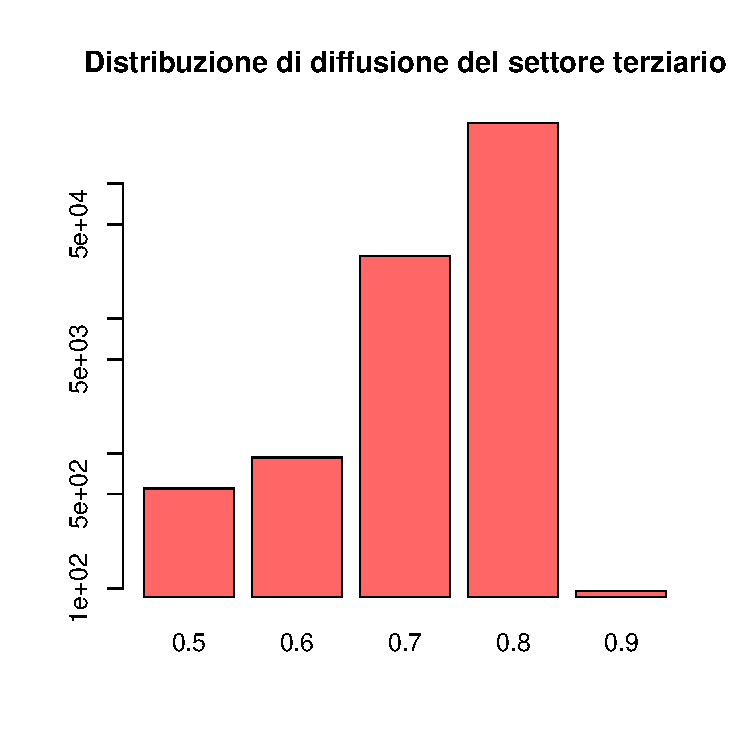
\includegraphics[width=0.4\linewidth]{../FinalResults/Images/Data_exploration_plots/barlpot_service}}}%
	\qquad
	\subfloat[Distribuzione dell'attributo state, l'etichetta dei nostri sample.]{{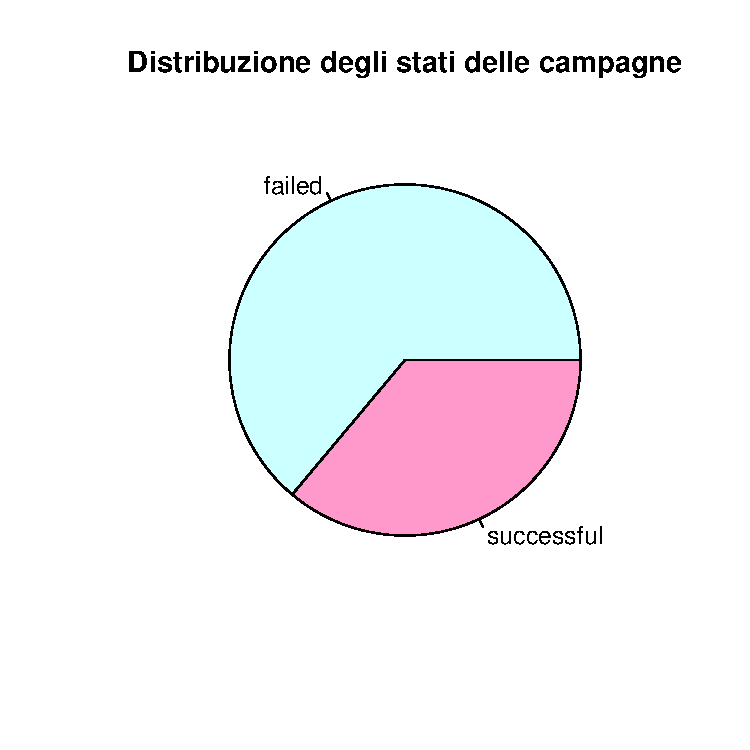
\includegraphics[width=0.4\linewidth]{../FinalResults/Images/Data_exploration_plots/pie_state}}}%
	\caption{}%
	\label{fig:piestate}%
\end{figure}

È stata infine prodotta la matrice di correlazione (mostrata in Figura \ref{fig:corrplot}) tra i vari attributi del dataset; come previsto, è emersa una evidente correlazione tra il paese in cui il progetto viene creato e i campi relativi al GDP pro capite e alla percentuale di diffusione del settore terziario nello stato. Questo poichè questi valori provengono da un dataset esterno joinato al dataset dei progetti Kickstarter proprio sul campo nazione. Dalla matrice non emergono altre correlazioni rilevanti tra i restanti attributi del dataset.

\begin{figure}
	\centering
	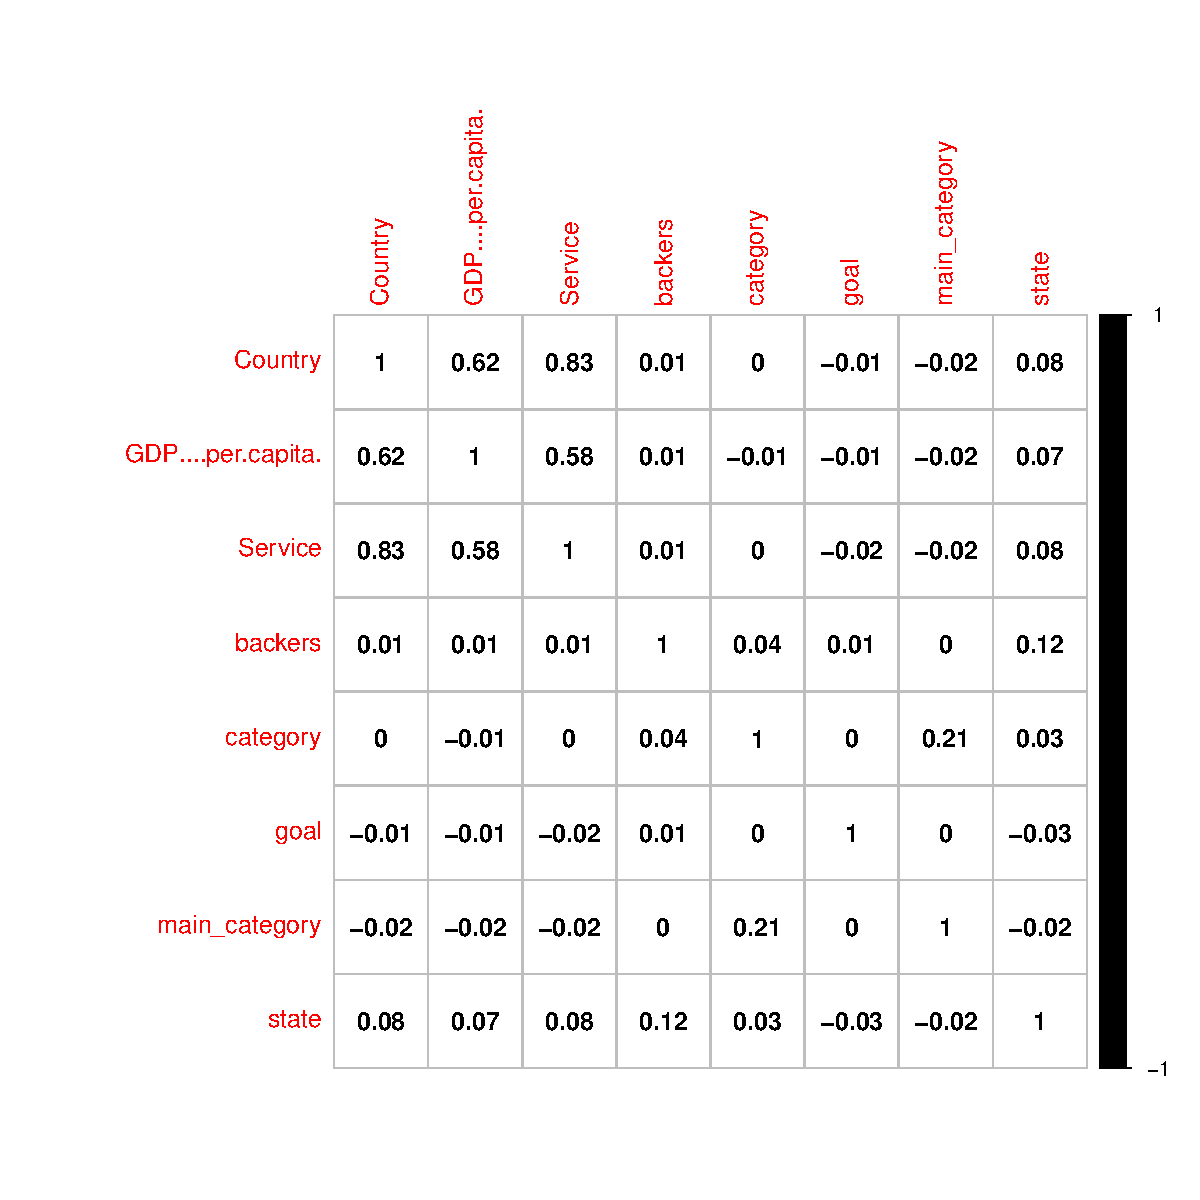
\includegraphics[width=1\linewidth]{../FinalResults/Images/Data_exploration_plots/corrplot}
	\caption{Matrice di correlazione tra le feature del dataset.}
	\label{fig:corrplot}
\end{figure}

\section{Modelli di Machine Learning utilizzati}
Al fine di avere una misura di riferimento per i modelli che saranno proposti successivamente, è stato prodotto un modello baseline, che si limita a rispondere sempre failed ad ogni sottomissione di un sample. La risposta risulta essere sempre failed in quanto, dall'analisi esplorativa dei dati effettuata in precedenza, è emerso che il valore di etichettatura più frequente era prorpio il fallimento del progetto.\\
In Figura \ref{fig:baselineperformance} e nella Tabella \ref{tab:acc_state} sono riportate le misure di performance ottenute con questo modello a seguito dell'operazione di 10 fold cross validation; notiamo come i valori di accuratezza e precisione si uniformino al valore di  probabilità dell'etichettatura failed nel dataset, mentre la recall rimanga ovviamente fissa ad 1.\\
Le curve ROC associate a questo modello, ripotate in Figura \ref{fig:baselineROC}, restituiscono un valore della Area Under Curve (AUC) molto variabile: ciò è dovuto dalla diversa distribuzione dei sample con etichettatura failed all'interno dei testset prodotti dal porcesso di 10-fold cross validation.
\begin{table}
	\caption{Tabella che riporta rispettivamente media e deviazione standard delle misure in Figura \ref{fig:baselineperformance}.}
	\label{tab:baselineperformance}
	\centering
	\begin{tabular}{c|c|c}
		Accuracy & 0.6389 & 0.0028 \\ 
		Precision & 0.6389 & 0.0027 \\
		Recall & 1 & 0 \\
		F1Measure & 0.7797 & 0.0020 \\
	\end{tabular}
\end{table} 
\begin{figure}
	\centering
	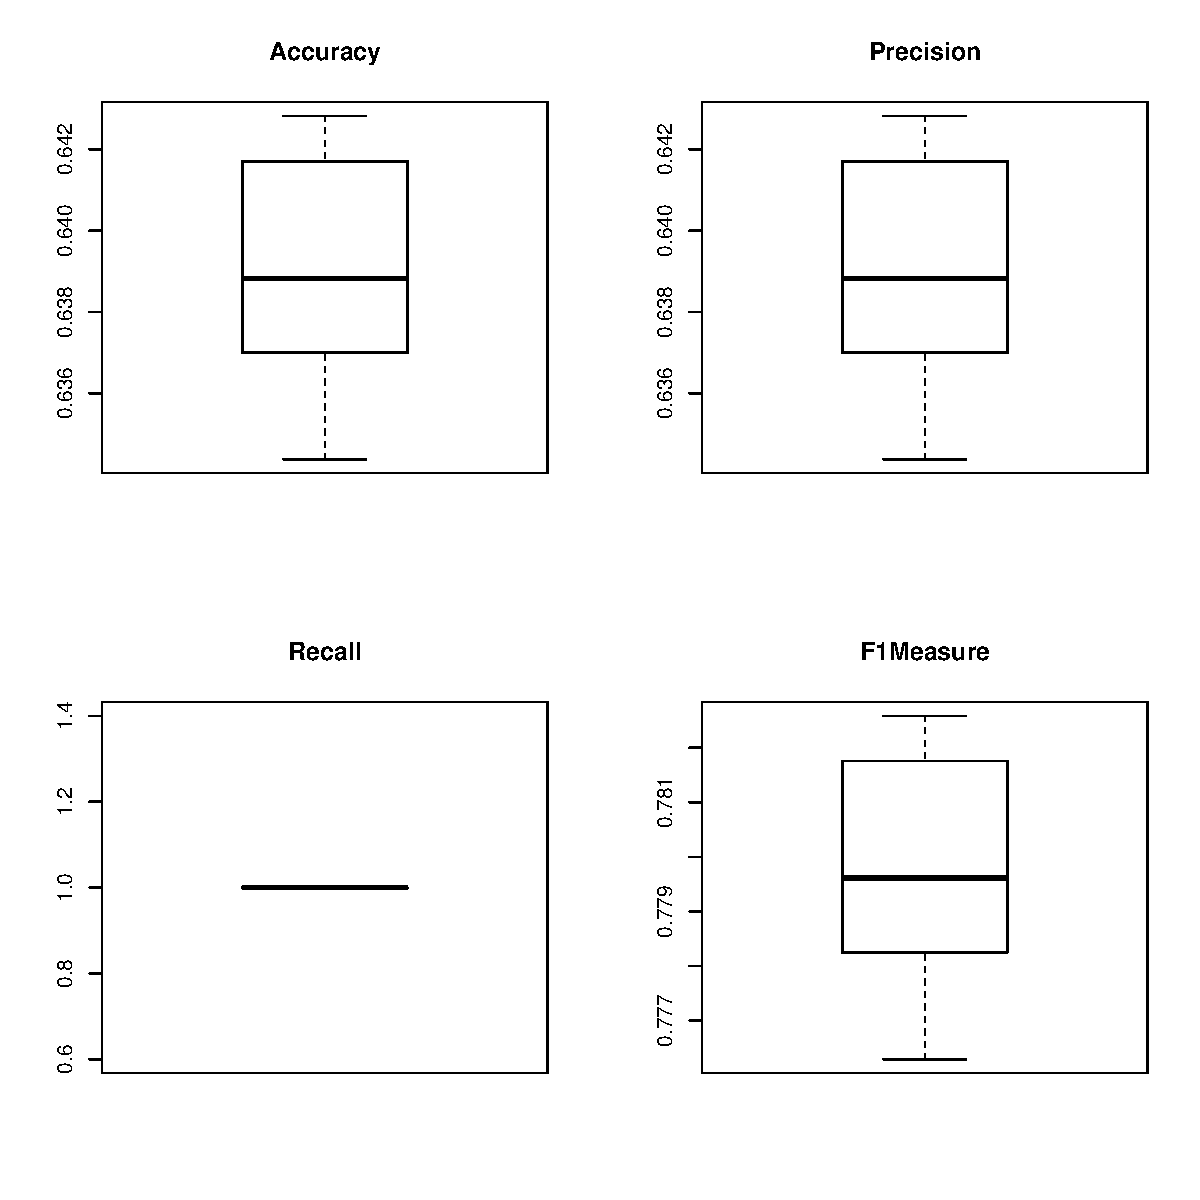
\includegraphics[width=0.7\linewidth]{../FinalResults/Baseline_performance}
	\caption{Boxplot relativi alle misure di performance del modello baseline.}
	\label{fig:baselineperformance}
\end{figure}

\begin{figure}
	\centering
	\subfloat{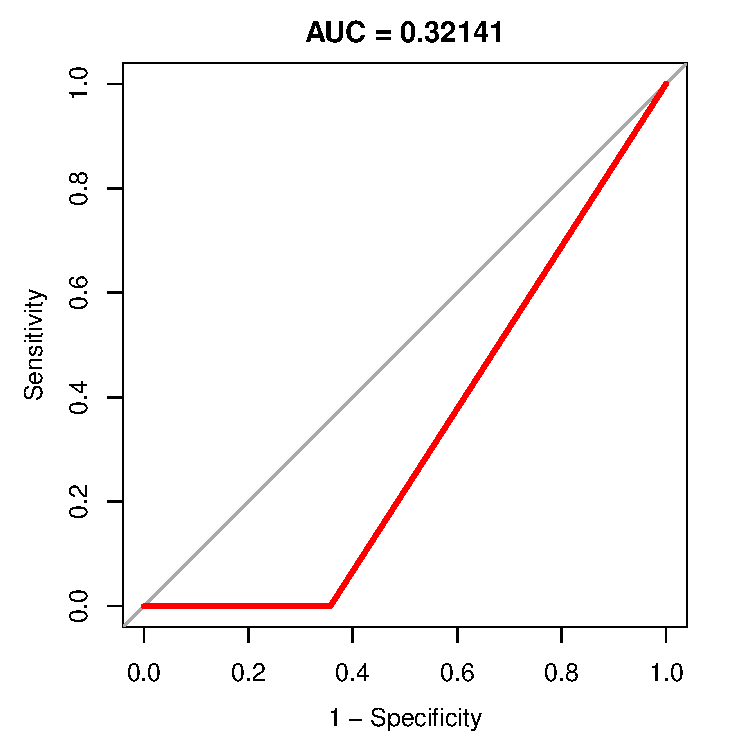
\includegraphics[width=0.3\linewidth]{../FinalResults/Images/baseline/auc_1.pdf}}\quad
	\subfloat{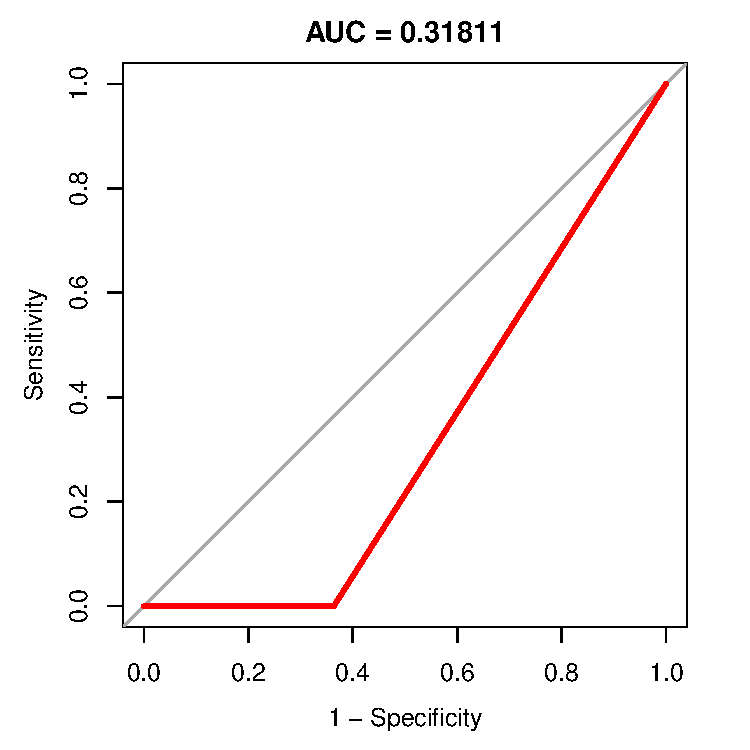
\includegraphics[width=0.3\linewidth]{../FinalResults/Images/baseline/auc_2.pdf}}\quad
	\subfloat{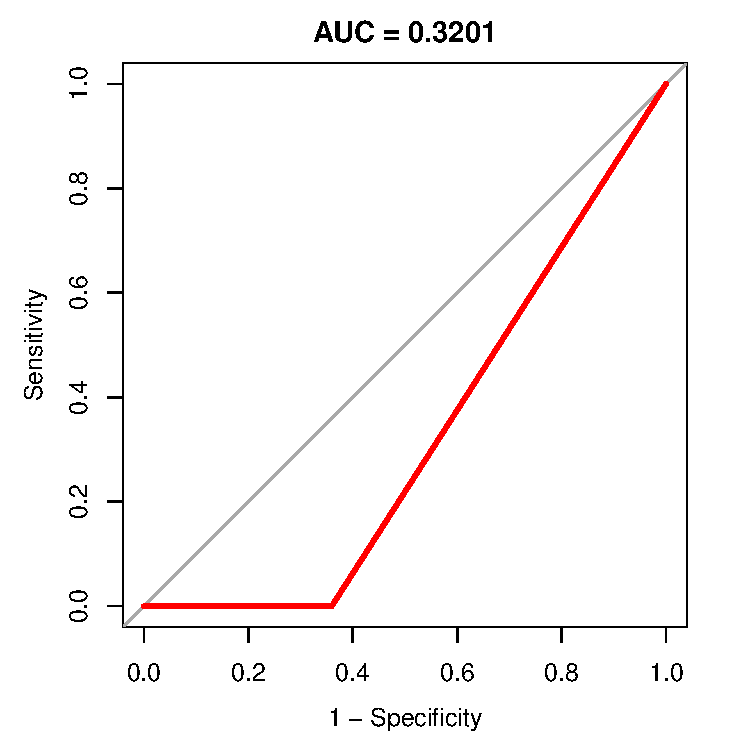
\includegraphics[width=0.3\linewidth]{../FinalResults/Images/baseline/auc_3.pdf}}\quad
	\subfloat{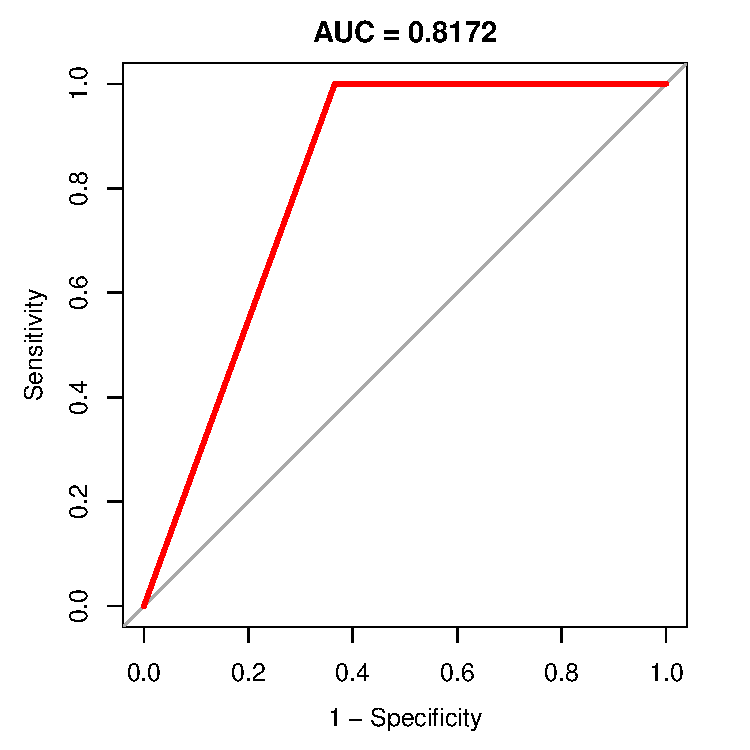
\includegraphics[width=0.3\linewidth]{../FinalResults/Images/baseline/auc_4.pdf}}\quad
	\subfloat{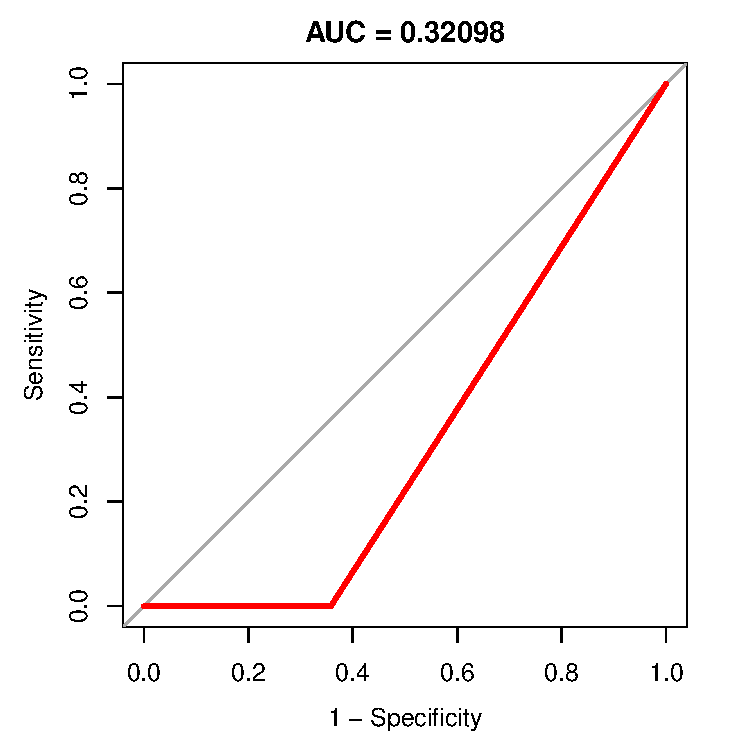
\includegraphics[width=0.3\linewidth]{../FinalResults/Images/baseline/auc_5.pdf}}\quad
	\subfloat{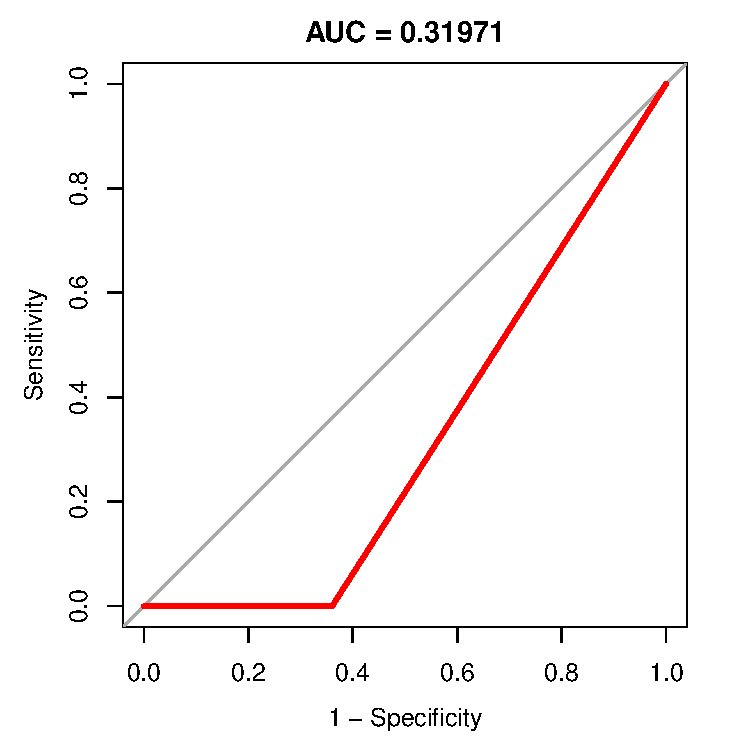
\includegraphics[width=0.3\linewidth]{../FinalResults/Images/baseline/auc_6.pdf}}\quad
	\subfloat{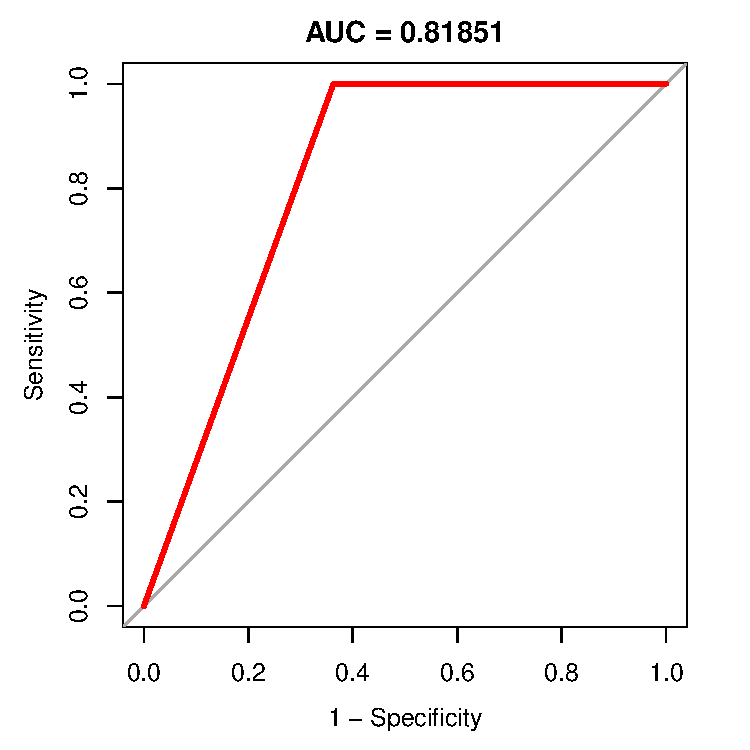
\includegraphics[width=0.3\linewidth]{../FinalResults/Images/baseline/auc_7.pdf}}\quad
	\subfloat{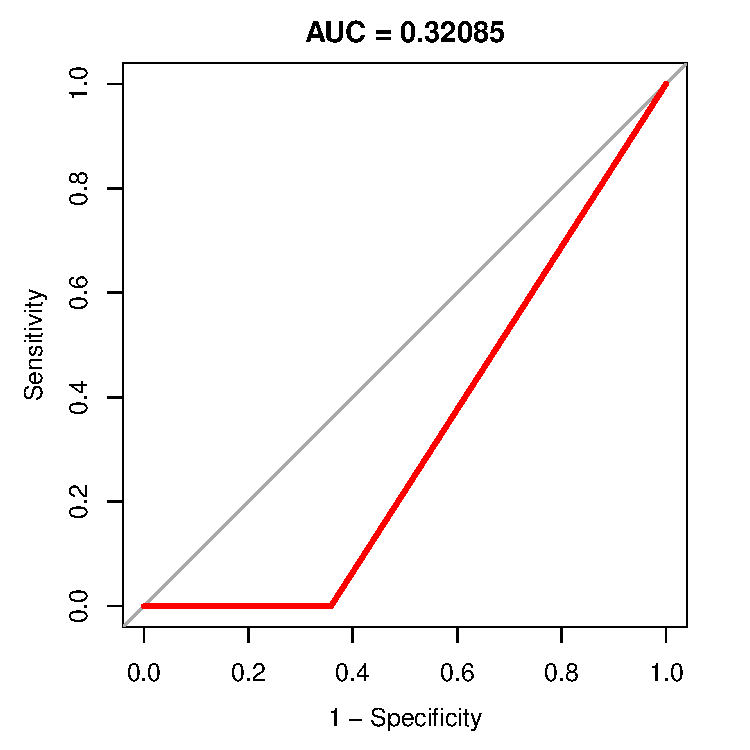
\includegraphics[width=0.3\linewidth]{../FinalResults/Images/baseline/auc_8.pdf}}\quad
	\subfloat{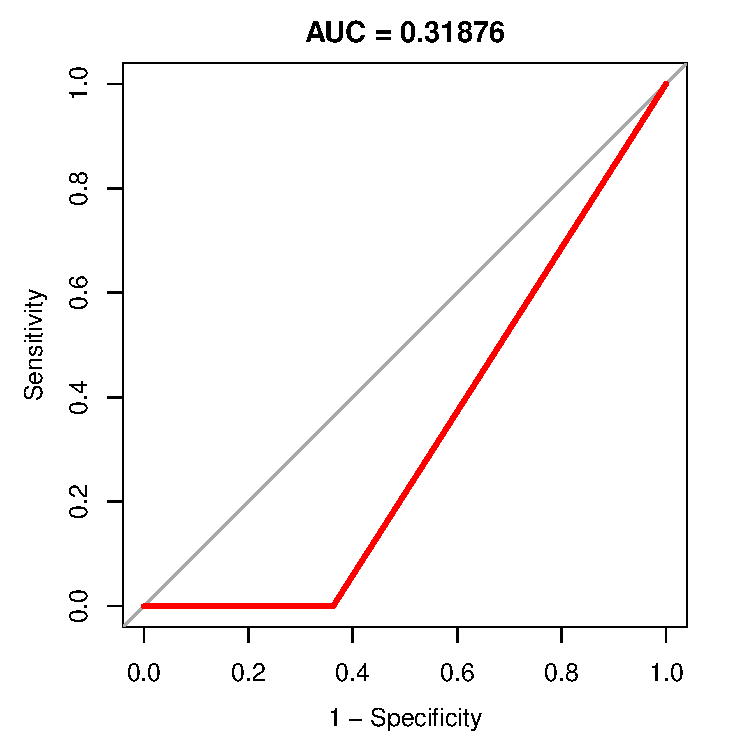
\includegraphics[width=0.3\linewidth]{../FinalResults/Images/baseline/auc_9.pdf}}\quad
	\subfloat{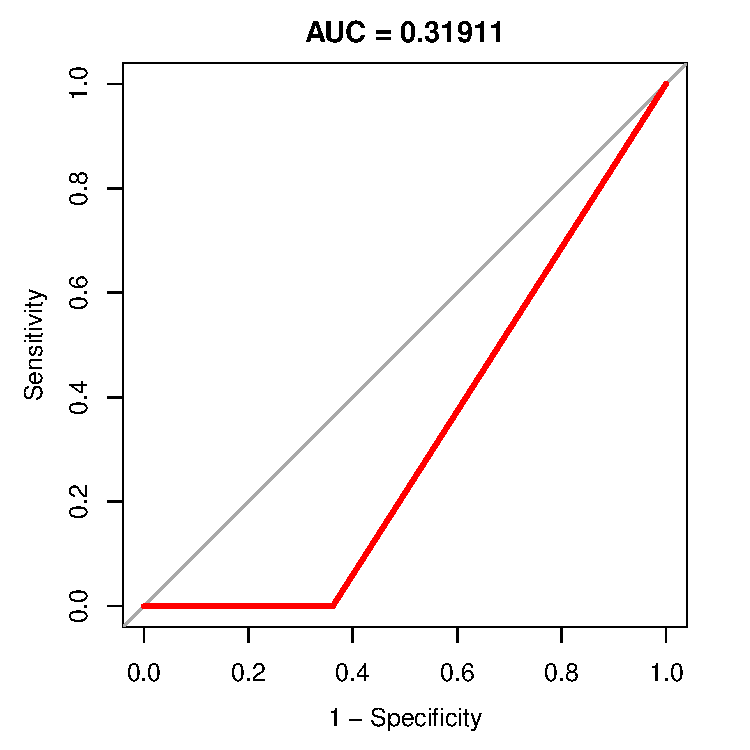
\includegraphics[width=0.3\linewidth]{../FinalResults/Images/baseline/auc_10.pdf}}\quad
	\caption{Curve ROC del modello baseline risultanti dal processo di 10-fold cross validation.}
	\label{fig:baselineROC}
\end{figure}       

\subsection{Alberi decisionali}
Gli alberi decisionali sono modelli utilizzati per il Machine Learning che basano la loro tecnica di predizione su un albero etichettato, in cui ad ogni nodo viene presa la decisione del ramo in cui proseguire in base al valore dell'attributo con cui il nodo è etichettato. Al termine di questo albero le foglie sono etichettate con il valore dell'attributo su cui si sta facendo predizione, nel nostro caso l'attributo state. Gli alberi implementati dalla libreria R texttt{rpart} permettono di valutare una serie di parametri, tra cui l'attributo cp, che permettono di regolare le dimensioni dell'albero prodotto e migliorarne le performance, riducendo, per quanto possibile, l'overfitting del modello.
Inizialmente è stato creato un albero che non sfruttava l'attributo backer del dataset, in quanto abbiamo immaginato che questo valore fosse di difficile stima per un utente che volesse inserire un nuovo progetto sulla piattaforma. L'albero generato si è però mostrato deludente, con performance paragonabili al modello baseline, come mostrato in Figura \ref{fig:treenbperformance} e in Tabella \ref{tab:treenbperformance}.
\begin{table}
	\caption{Tabella che riporta rispettivamente media e deviazione standard delle misure in Figura \ref{fig:treenbperformance}.}
	\label{tab:treenbperformance}
	\centering
	\begin{tabular}{c|c|c}
		Accuracy & 0.6814 & 0.0019 \\ 
		Precision & 0.7084 & 0.0036 \\
		Recall & 0.8521 & 0.0084 \\
		F1Measure & 0.7736 & 0.0024 \\
	\end{tabular}
\end{table}
\begin{figure}
	\centering
	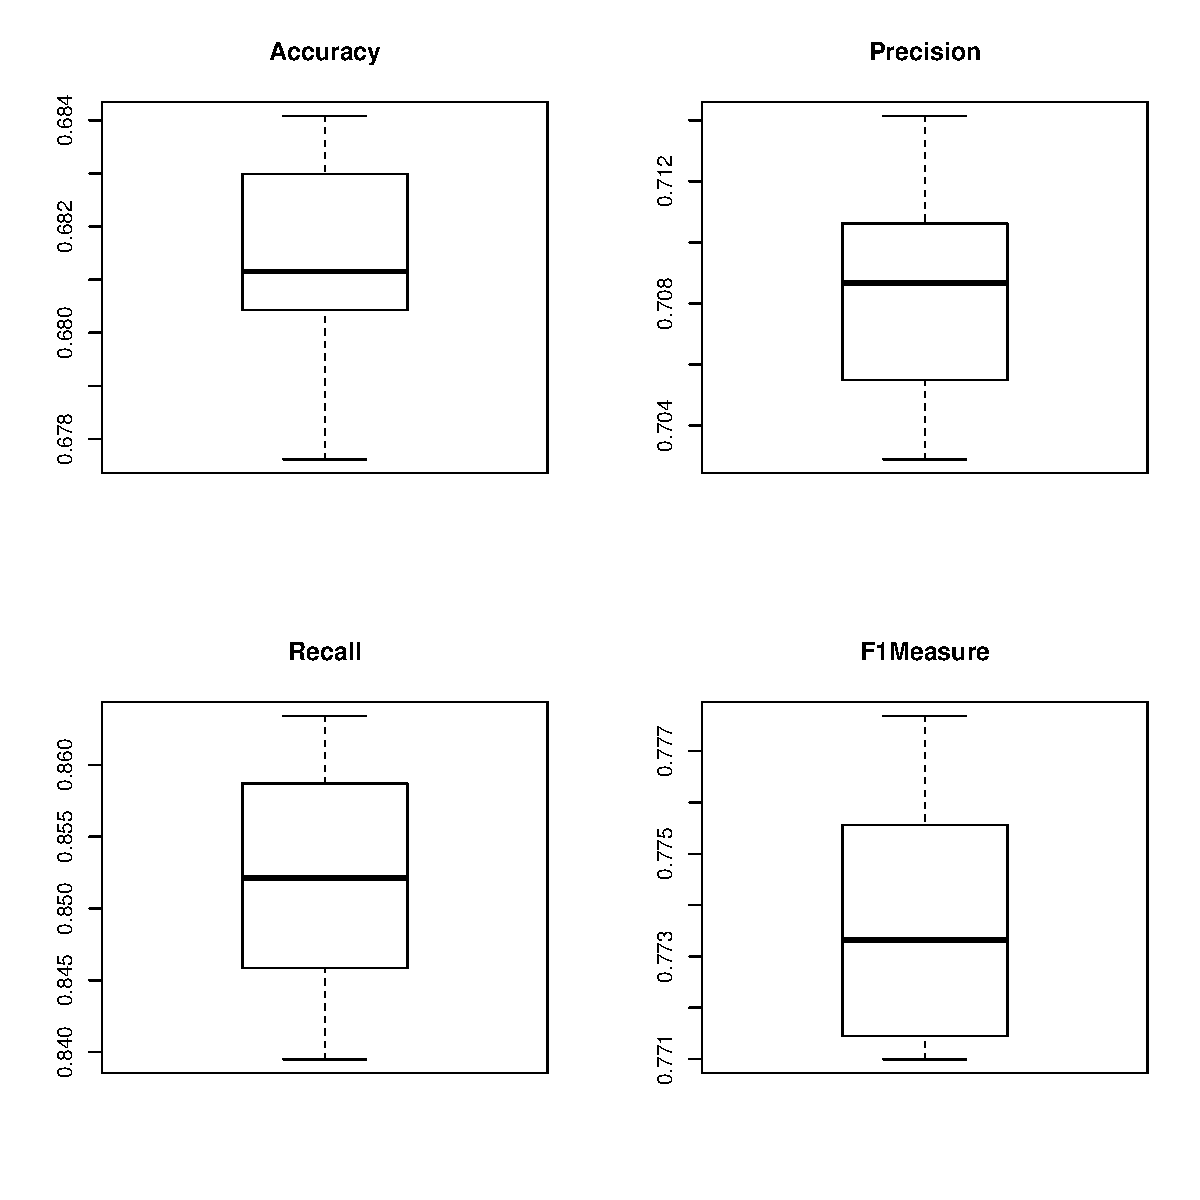
\includegraphics[width=0.7\linewidth]{../FinalResults/TreeNB_performance}
	\caption{Boxplot relativi alle misure di performance dell'albero di decisione senza l'utilizzo della feature backer.}
	\label{fig:treenbperformance}
\end{figure}
Le curve ROC relative a questo modello (riportate in Figura \ref{fig:treeNBROC}) sono risultate essere molto simili nelle varie iterazioni, mostrando un maggiore livello di solidità circa la composizione del trainset e del testset rispetto al modello baseline.
\begin{figure}
	\centering
	\subfloat{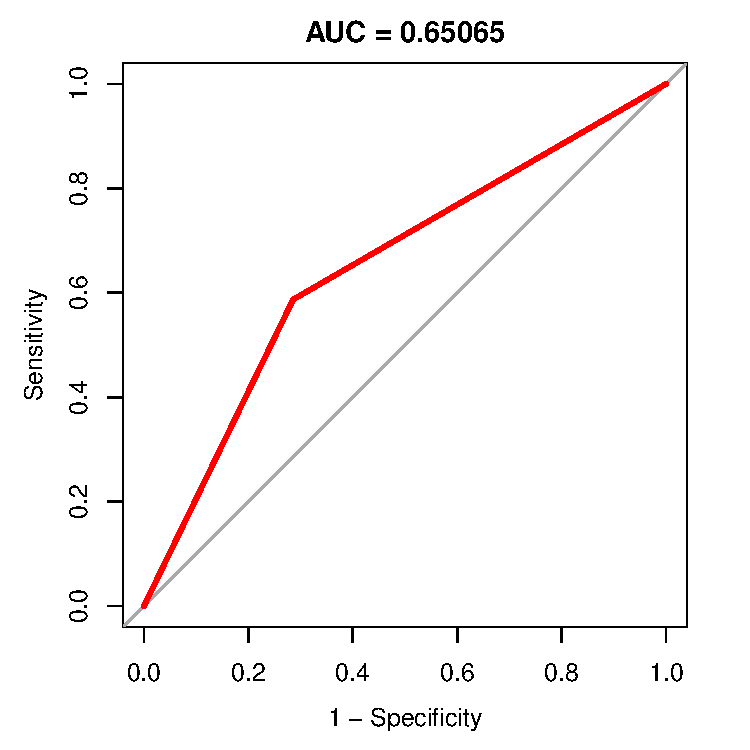
\includegraphics[width=0.3\linewidth]{../FinalResults/Images/treeNB/auc_1.pdf}}\quad
	\subfloat{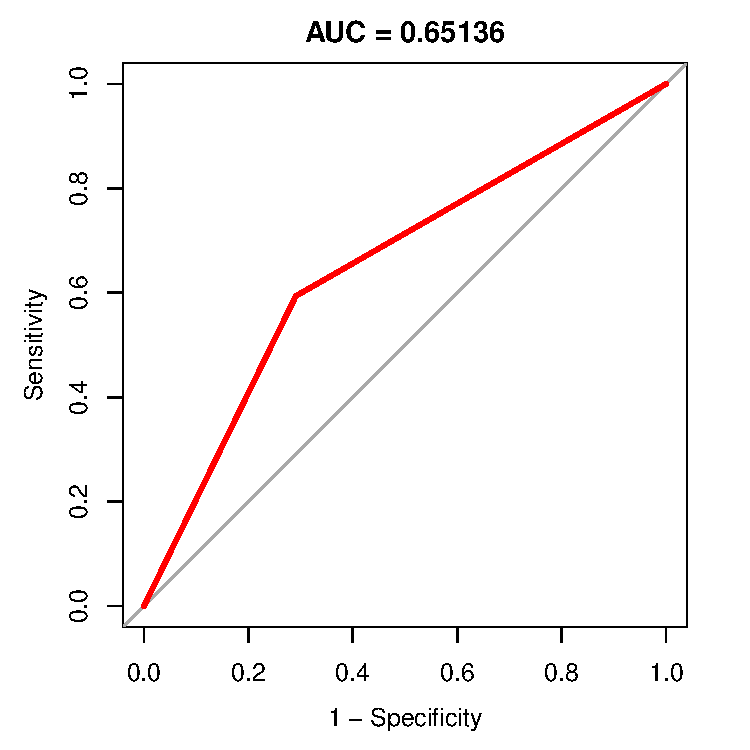
\includegraphics[width=0.3\linewidth]{../FinalResults/Images/treeNB/auc_2.pdf}}\quad
	\subfloat{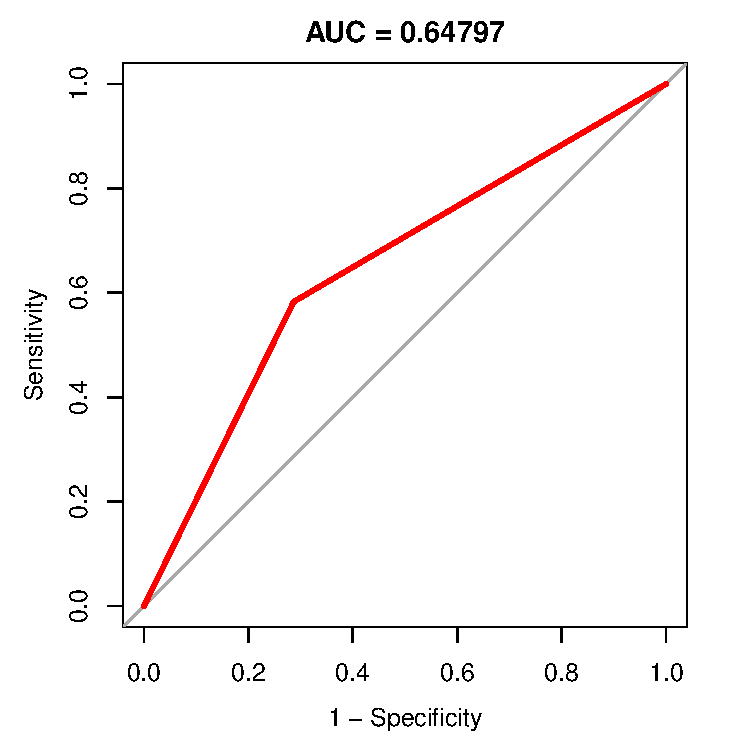
\includegraphics[width=0.3\linewidth]{../FinalResults/Images/treeNB/auc_3.pdf}}\quad
	\subfloat{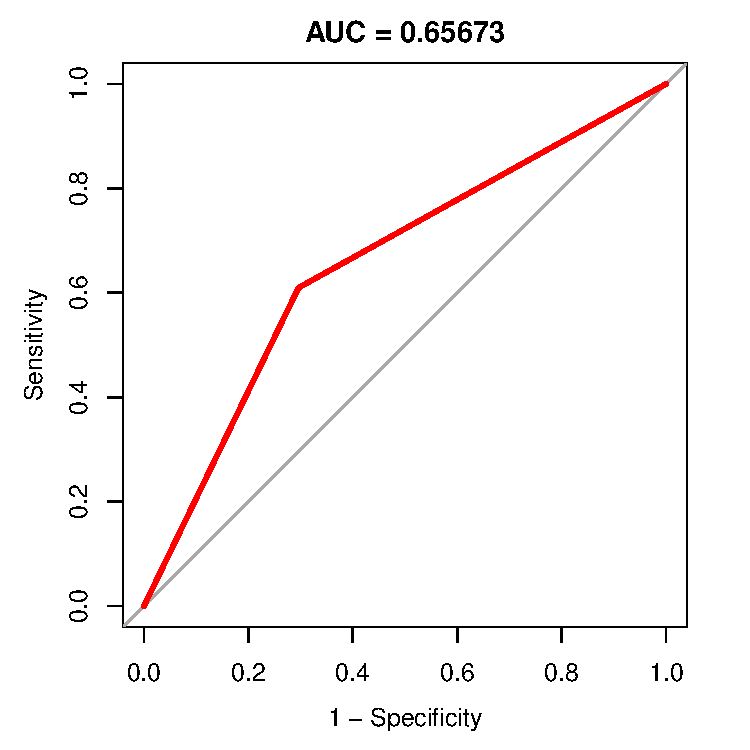
\includegraphics[width=0.3\linewidth]{../FinalResults/Images/treeNB/auc_4.pdf}}\quad
	\subfloat{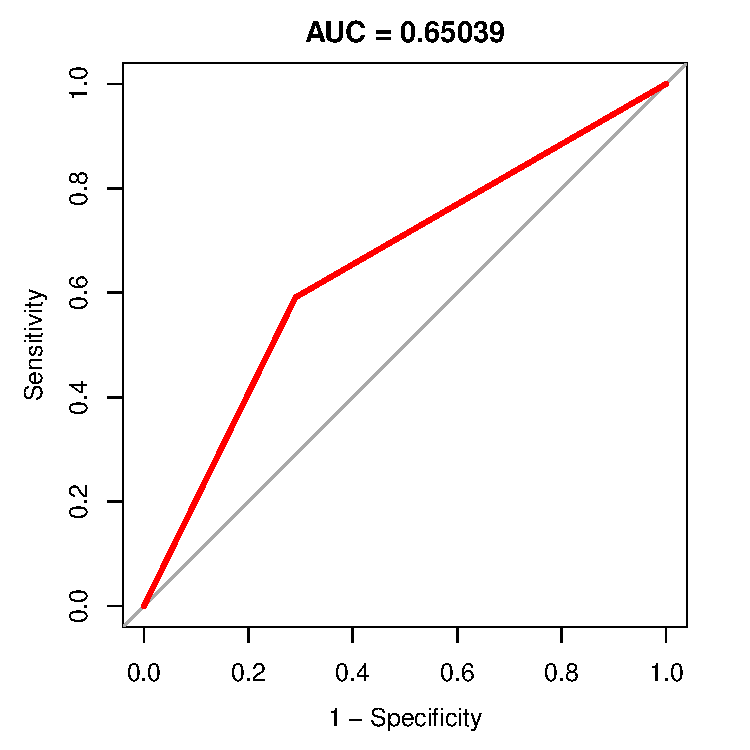
\includegraphics[width=0.3\linewidth]{../FinalResults/Images/treeNB/auc_5.pdf}}\quad
	\subfloat{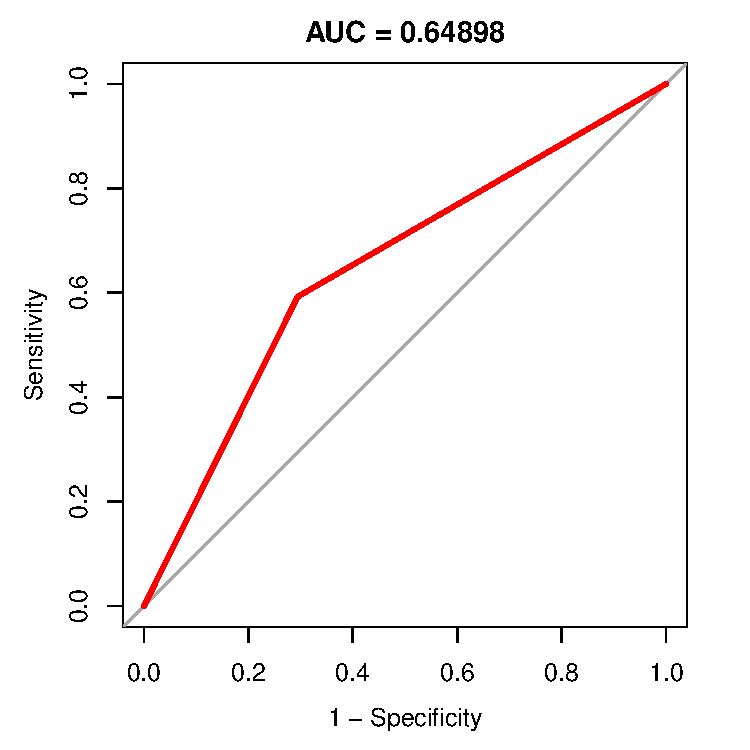
\includegraphics[width=0.3\linewidth]{../FinalResults/Images/treeNB/auc_6.pdf}}\quad
	\subfloat{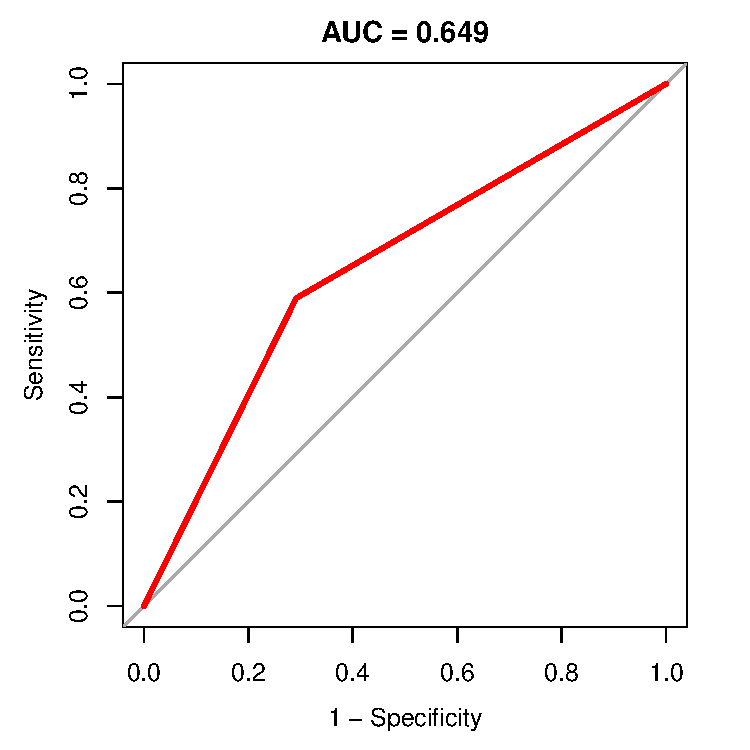
\includegraphics[width=0.3\linewidth]{../FinalResults/Images/treeNB/auc_7.pdf}}\quad
	\subfloat{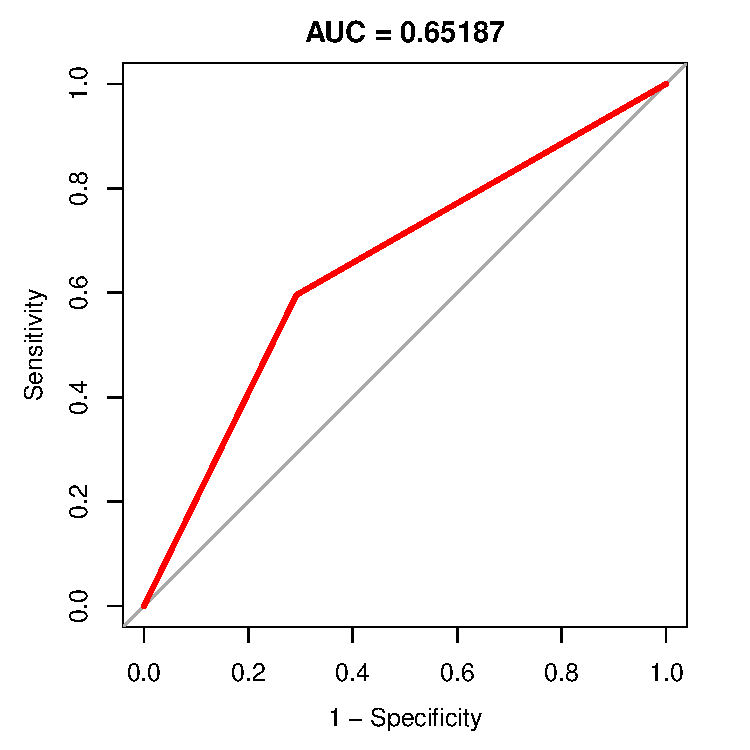
\includegraphics[width=0.3\linewidth]{../FinalResults/Images/treeNB/auc_8.pdf}}\quad
	\subfloat{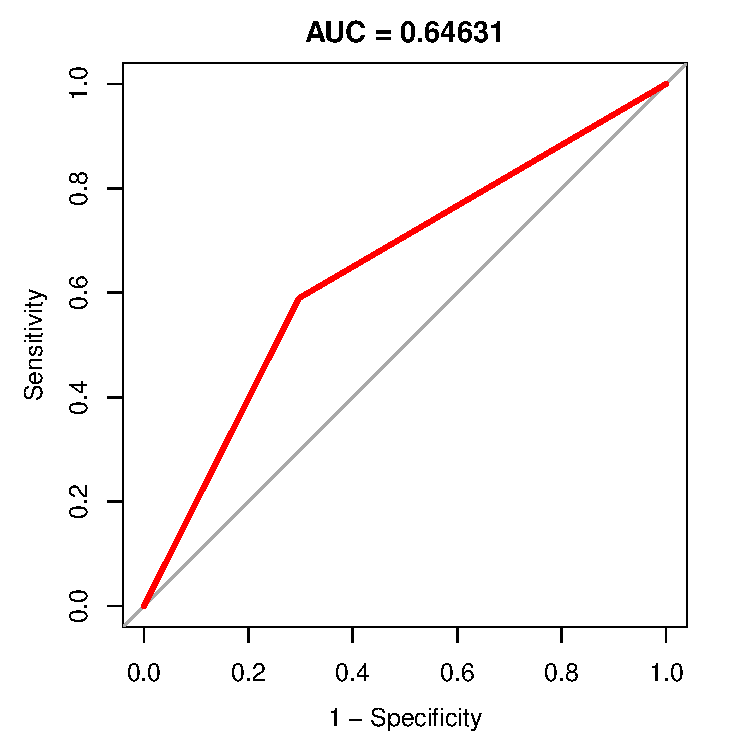
\includegraphics[width=0.3\linewidth]{../FinalResults/Images/treeNB/auc_9.pdf}}\quad
	\subfloat{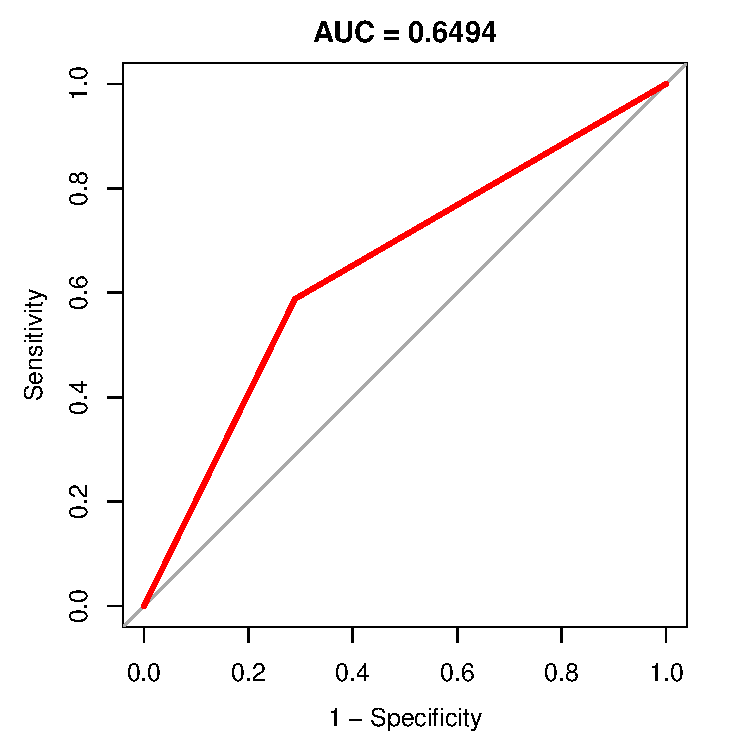
\includegraphics[width=0.3\linewidth]{../FinalResults/Images/treeNB/auc_10.pdf}}\quad
	\caption{Curve ROC del modello ad albero senza l'utilizzo della feature baker risultanti dal processo di 10-fold cross validation.}
	\label{fig:treeNBROC}
\end{figure}  
\newpage
E' stato quindi deciso di sfruttare tutte le feature disponibili, supponendo che per futuri progetti non ancora realizzati sarà possibile stimare il valore dei backer tramite l'utilizzo di modelli di regressione lineare. L'albero prodotto dal processo di addestramento è mostrato in Figura \ref{fig:tree}. Le performance ottenute dal nuovo modello sono decisamente superiori al precedente, come mostrato in nella Tabella e in Figura.\\
\begin{figure}
	\centering
	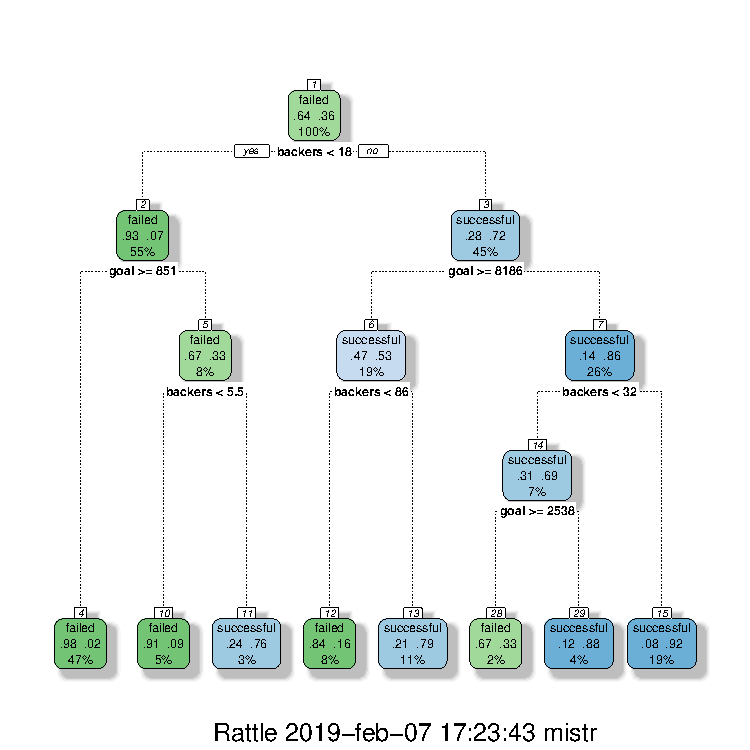
\includegraphics[width=0.9\linewidth]{../FinalResults/tree}
	\caption{Albero prodotto dal processo di addestramento con tutte le feature del dataset.}
	\label{fig:tree}
\end{figure}
Le feature utilizzate dal modello sono esclusivamente il numero di backer e il goal del progetto, gli altri campi del dataset non sono utilizzati per la classificazione. Ciononostante le performance ottenute da questo modello (riportate nella Tabella \ref{tab:treeperformance} e in Figura \ref{fig:treeperformance}) si sono rivelate più che discrete, superando nettamente il modello baseline proposto. La scarsissima varianza dei valori durante il processo di 10-fold cross validation mostra come il modello prodotto sia solido e non sensibile a eventuali eterogeneità di distribuzione di tuple etichettate come fallite o riuscite. Questo si ripercuote anche sulle curve ROC, riportate in Figura \ref{fig:treeROC}, il cui andamento è pressoché identico durante tutte le 10 iterazioni di validazione.

\begin{table}
	\caption{Tabella che riporta rispettivamente media e deviazione standard delle misure in Figura \ref{fig:treeperformance}.}
	\label{tab:treeperformance}
	\centering
	\begin{tabular}{c|c|c}
		Accuracy & 0.9112 & 0.0021 \\ 
		Precision & 0.9376 & 0.0030 \\
		Recall & 0.9224 & 0.0019 \\
		F1Measure & 0.9299 & 0.0018 \\
	\end{tabular}
\end{table}
\begin{figure}
	\centering
	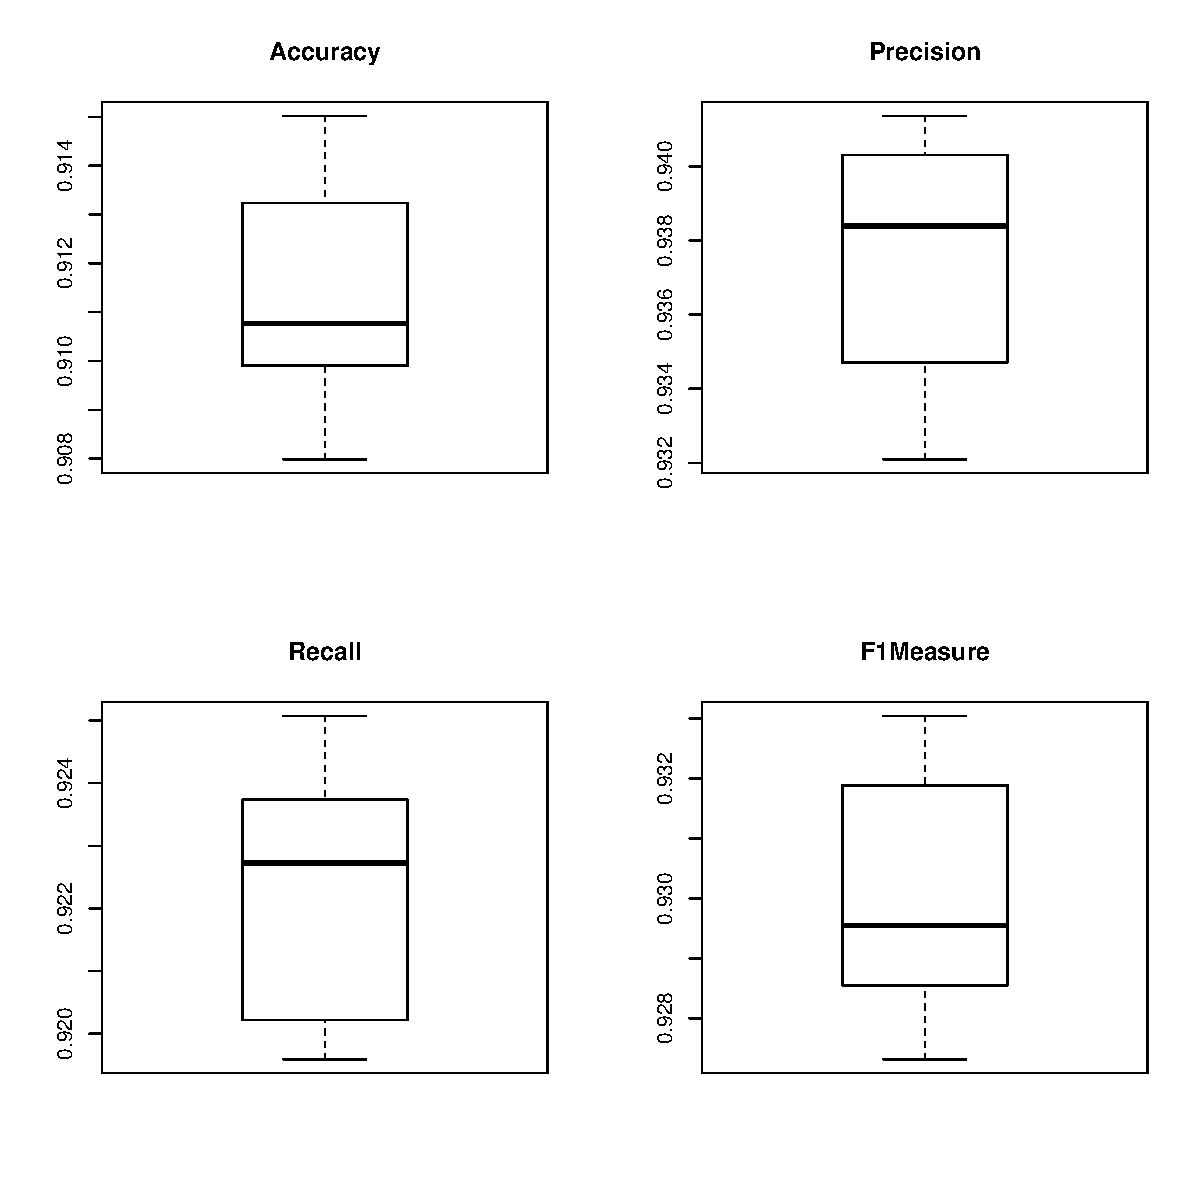
\includegraphics[width=0.7\linewidth]{../FinalResults/Tree_performance}
	\caption{Boxplot relativi alle misure di performance dell'albero di decisione con tutte le feature.}
	\label{fig:treeperformance}
\end{figure}
\begin{figure}
	\centering
	\subfloat{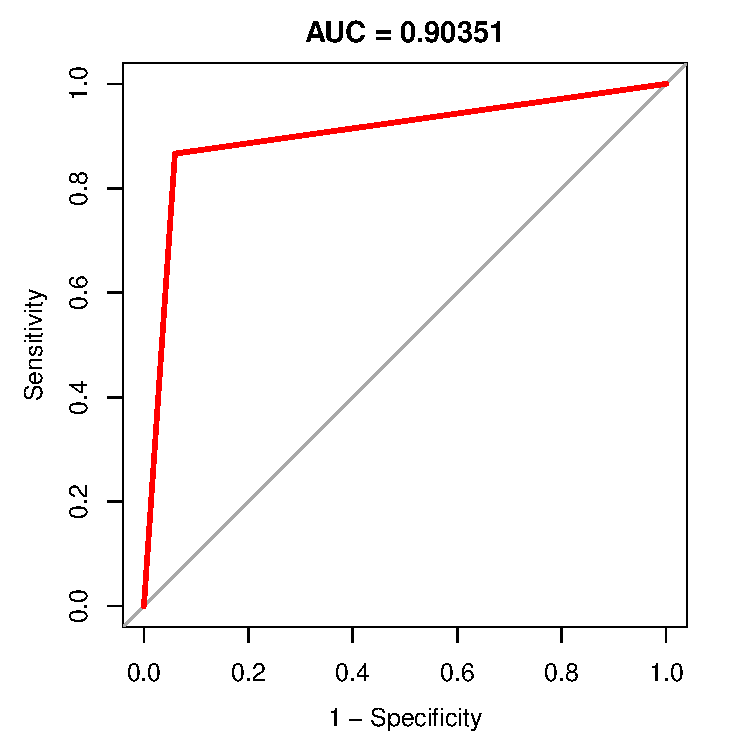
\includegraphics[width=0.3\linewidth]{../FinalResults/Images/tree/auc_1.pdf}}\quad
	\subfloat{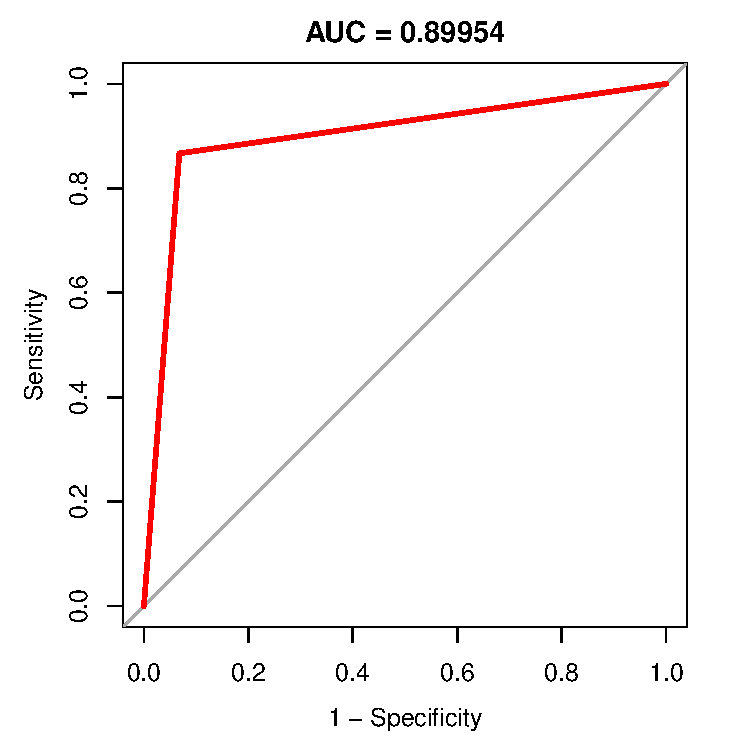
\includegraphics[width=0.3\linewidth]{../FinalResults/Images/tree/auc_2.pdf}}\quad
	\subfloat{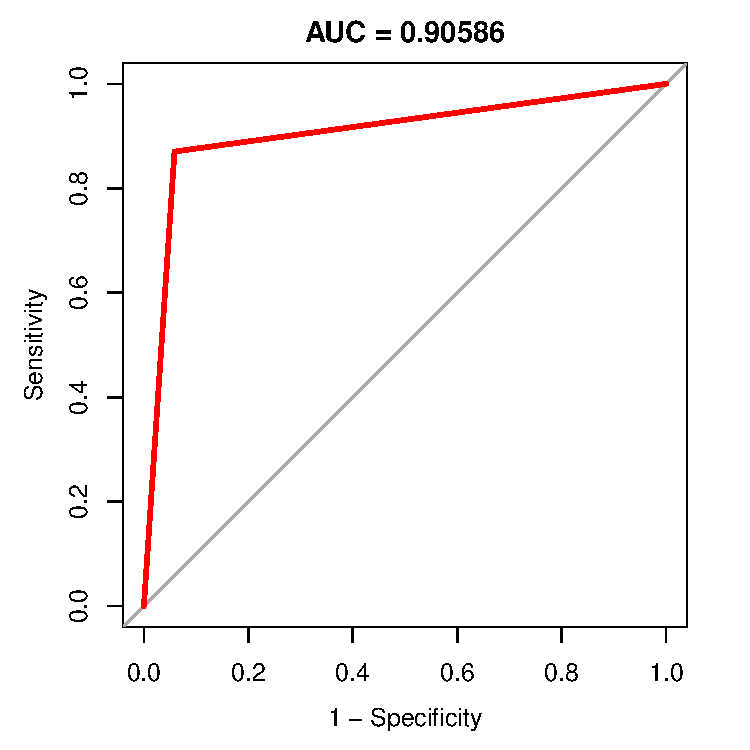
\includegraphics[width=0.3\linewidth]{../FinalResults/Images/tree/auc_3.pdf}}\quad
	\subfloat{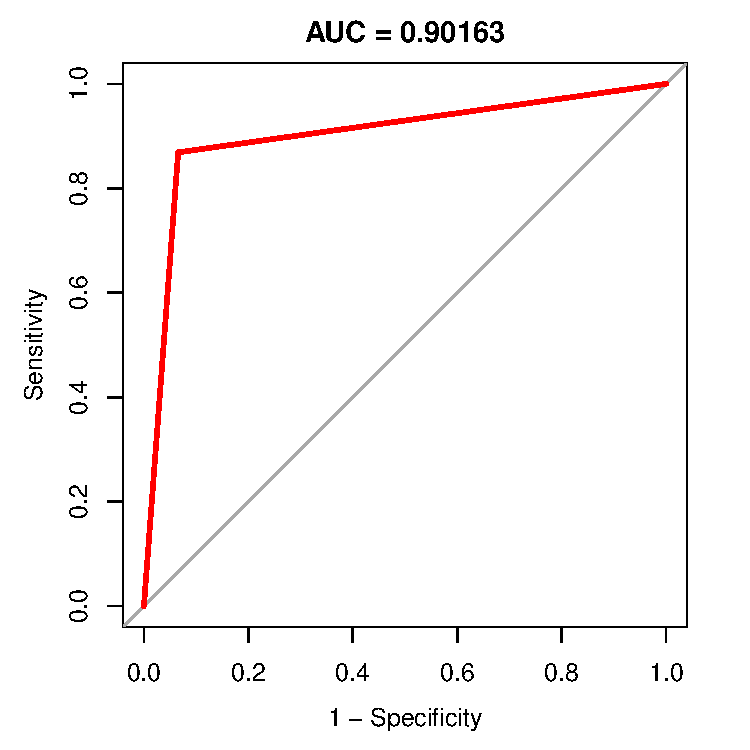
\includegraphics[width=0.3\linewidth]{../FinalResults/Images/tree/auc_4.pdf}}\quad
	\subfloat{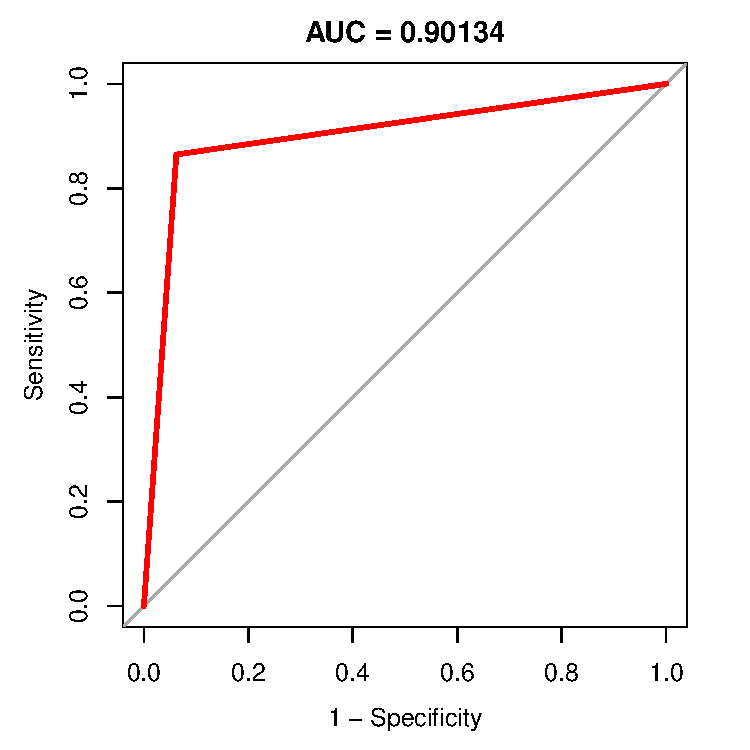
\includegraphics[width=0.3\linewidth]{../FinalResults/Images/tree/auc_5.pdf}}\quad
	\subfloat{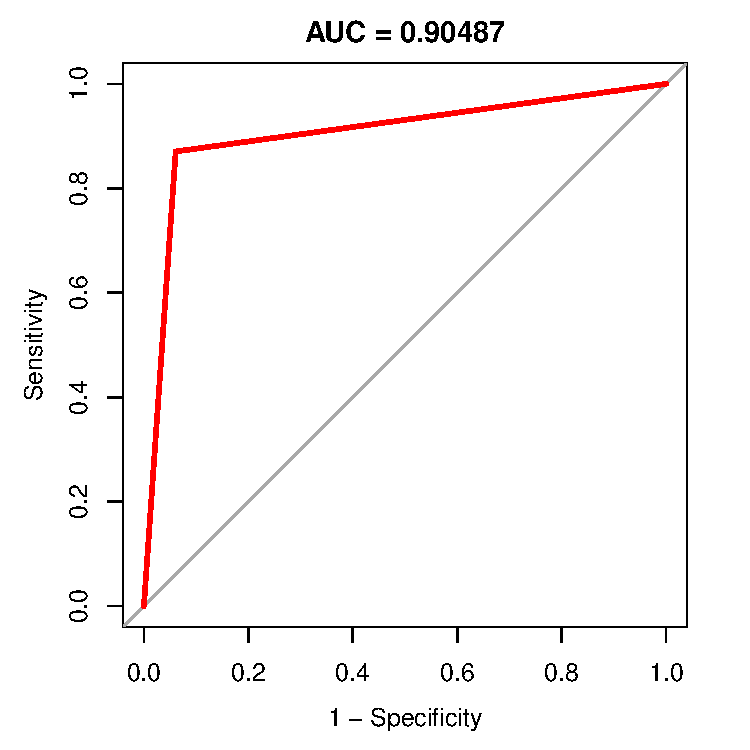
\includegraphics[width=0.3\linewidth]{../FinalResults/Images/tree/auc_6.pdf}}\quad
	\subfloat{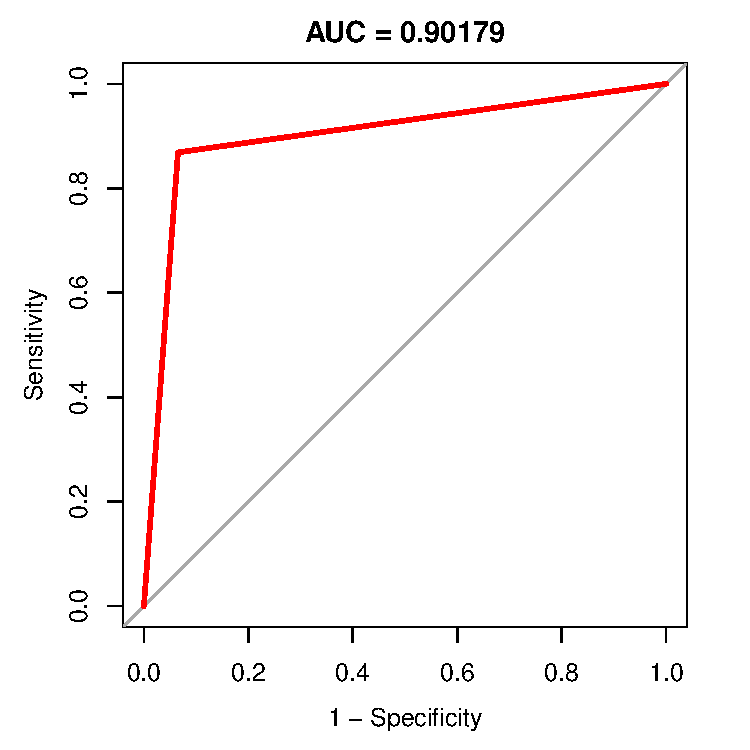
\includegraphics[width=0.3\linewidth]{../FinalResults/Images/tree/auc_7.pdf}}\quad
	\subfloat{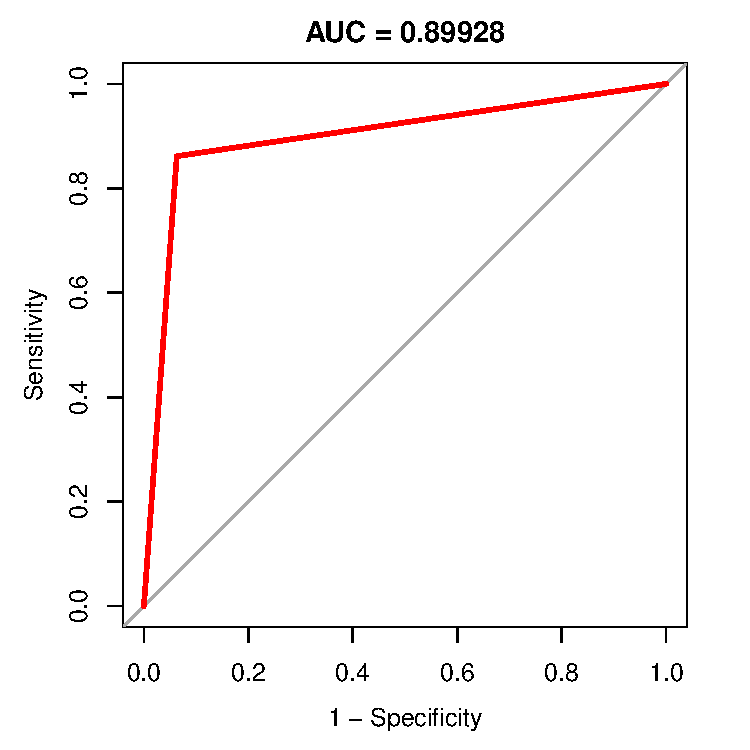
\includegraphics[width=0.3\linewidth]{../FinalResults/Images/tree/auc_8.pdf}}\quad
	\subfloat{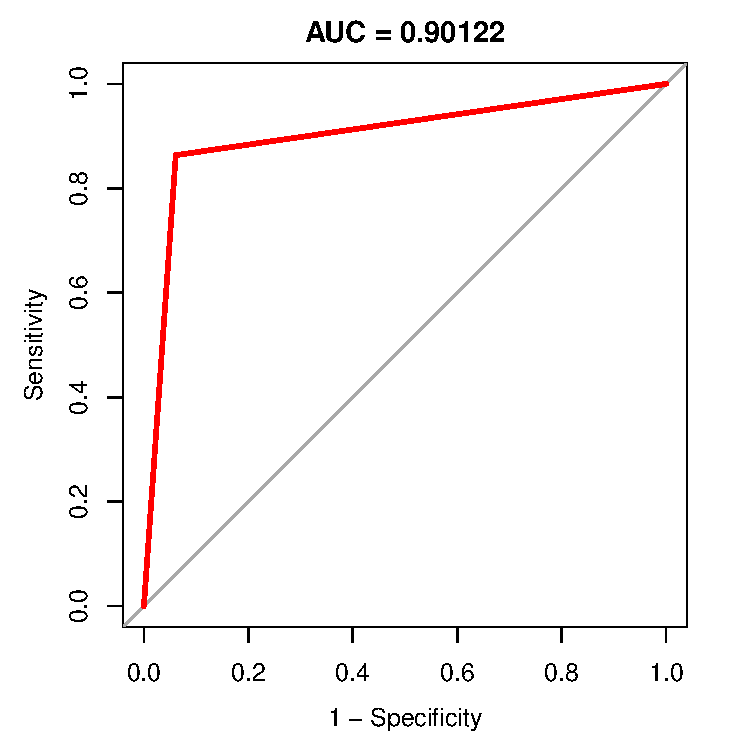
\includegraphics[width=0.3\linewidth]{../FinalResults/Images/tree/auc_9.pdf}}\quad
	\subfloat{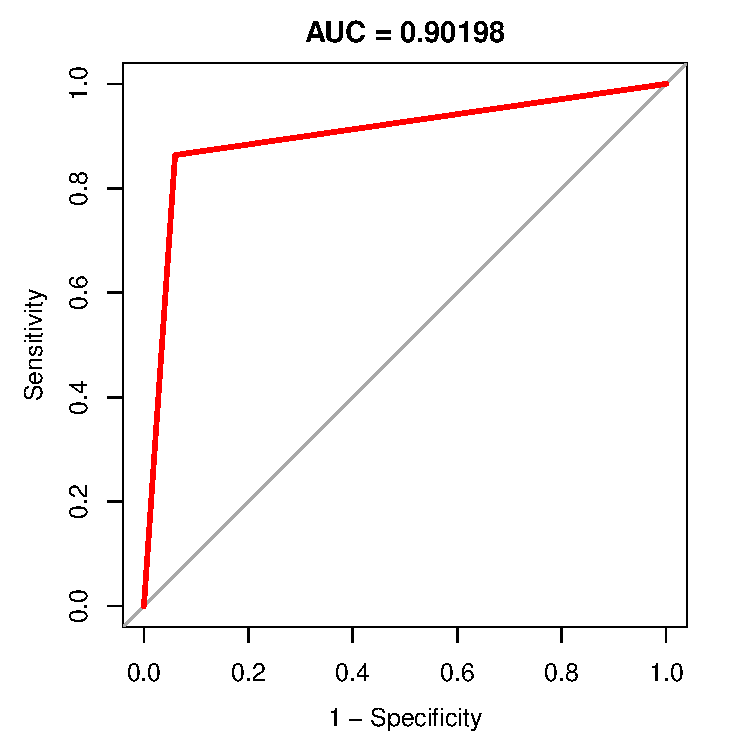
\includegraphics[width=0.3\linewidth]{../FinalResults/Images/tree/auc_10.pdf}}\quad
	\caption{Curve ROC del modello ad albero risultanti dal processo di 10-fold cross validation.}
	\label{fig:treeROC}
\end{figure}   

Infine, abbiamo valutato il parametro di complessità dell'albero prodotto. Il grafico (riportato in Figura \ref{fig:cptree}), seppur mostrando un valore di complessità molto basso, mostra come sia effettivamente possibile effettuare una potatura di alcuni rami pagando un costo in performance predittive infinitesimale. Abbiamo quindi deciso di effettuare la potatura dell'albero ponendo il valore del parametro cp a $0.015$, ottenendo così l'albero riportato in Figura \ref{fig:prunedtree}. Le misure di performance, non riportate di seguito per questioni di brevità, sono completamente assimilabili a quelle riportate per l'albero non potato.
\begin{figure}
	\centering
	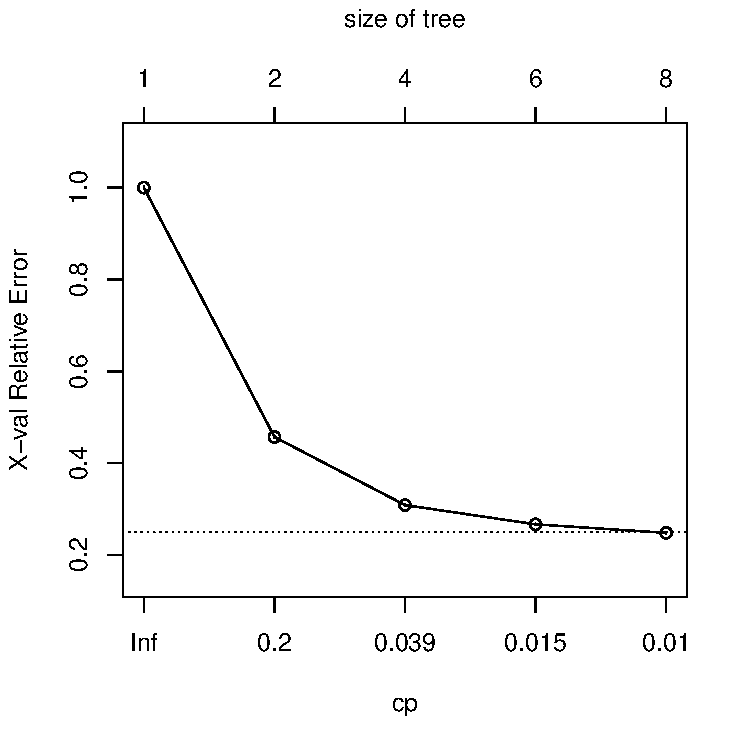
\includegraphics[width=0.7\linewidth]{../FinalResults/cptree}
	\caption{Grafico dell'andamento del parametro di complessità al crescere del numero di ramificazioni.}
	\label{fig:cptree}
\end{figure}
\begin{figure}
	\centering
	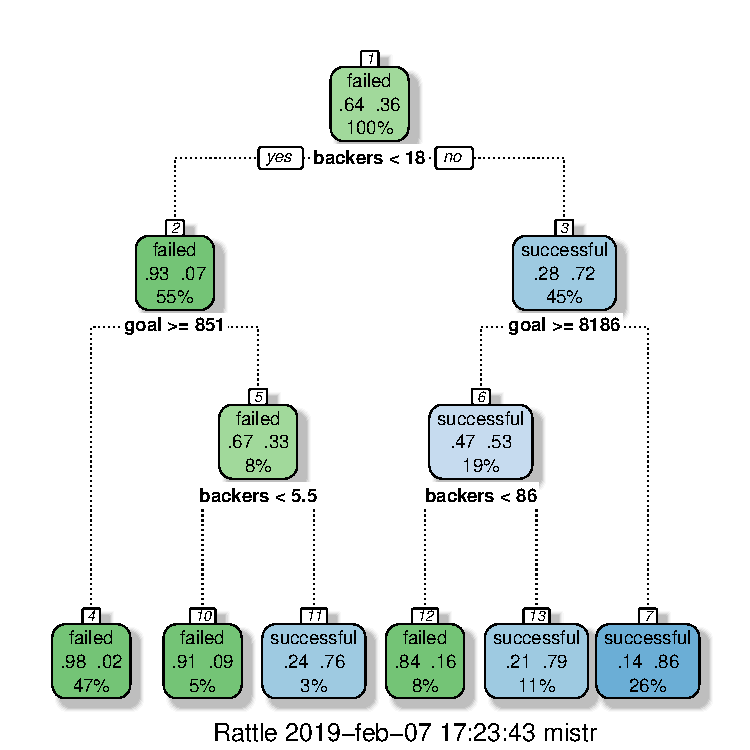
\includegraphics[width=0.7\linewidth]{../FinalResults/prunedtree}
	\caption{Albero risultante dalla potatura con valore del parametro cp pari a 0.015}
	\label{fig:prunedtree}
\end{figure}

\subsection{Naive Baies}
\subsection{Support Vector Machine}
\subsection{Reti neurali}
Le reti neurali sono un modello che si è rivelato non performare come sperato per il nostro caso di studio. L'assenza di conoscenza pregressa circa una possibile topologia della rete e l'abbondanza di parametri che influiscono sulla corretta convergenza dell'algoritmo di apprendimento ha portato alla impossibilità di produrre un modello funzionante. Sono stati effettuati numerosi test per trovare la corretta combinazione di parametri, modificando il numero di neuroni nascosti, il numero massimo di iterazioni del processo di learnig e il valore di learning rate della rete; seppur alcuni test su scala ridotta abbiano prodotto un modello funzionante e dalle performance accettabili (riportate in Tabella \ref{tab:nnperformance}), ogni tentativo di training della rete sull'intero dataset ha portato alla non convergenza del processo. Abbiamo quindi deciso di non includere questo modello nella nostra analisi, in quanto non è stato possibile replicare i risultati ottenuti su scala ridotta su tutto il dataset. Altri fattori che hanno contribuito all'esclusione di questo modello sono il lungo tempo di training della rete al crescere del numero di neuroni e di sample in input.

\begin{table}
	\caption{Tabella che riporta i valori delle misure di performance sulla rete trainata su 1000 sample del dataset.}
	\label{tab:nnperformance}
	\centering
	\begin{tabular}{c|c}
		Accuracy & 0.8953  \\ 
		Precision & 0.9808  \\
		Recall & 0.8521  \\
		F1Measure & 0.9119  \\
	\end{tabular}
\end{table}

\subsection{Confronto tra modelli}
\section{Conclusioni}